\documentclass[../DS05.tex]{subfiles}
\graphicspath{{./figures/}}

% \subimport{/home/nora/Documents/Enseignement/Prepa/bpep/exercices/DS/ondes_gravitationnelles/}{sujet.tex}
\begin{document}

\exercice[23]{Ondes gravitationnelles}
\enonce{
	Le prix Nobel 2017 a été remis aux responsables de l'expérience Ligo, qui a
	détecté des ondes gravitationnelles trois fois en un an. Cette expérience
	n'est pas la seule dans le monde. L'expérience franco-italienne Virgo a
	également détecté cette même année et pour la première fois des ondes
	gravitationnelles. Ces expériences exploitent le phénomène d'interférences
	lumineuses.
	\smallbreak
	\noindent
	\begin{minipage}[c]{.54\linewidth}
		~
		\begin{center}
			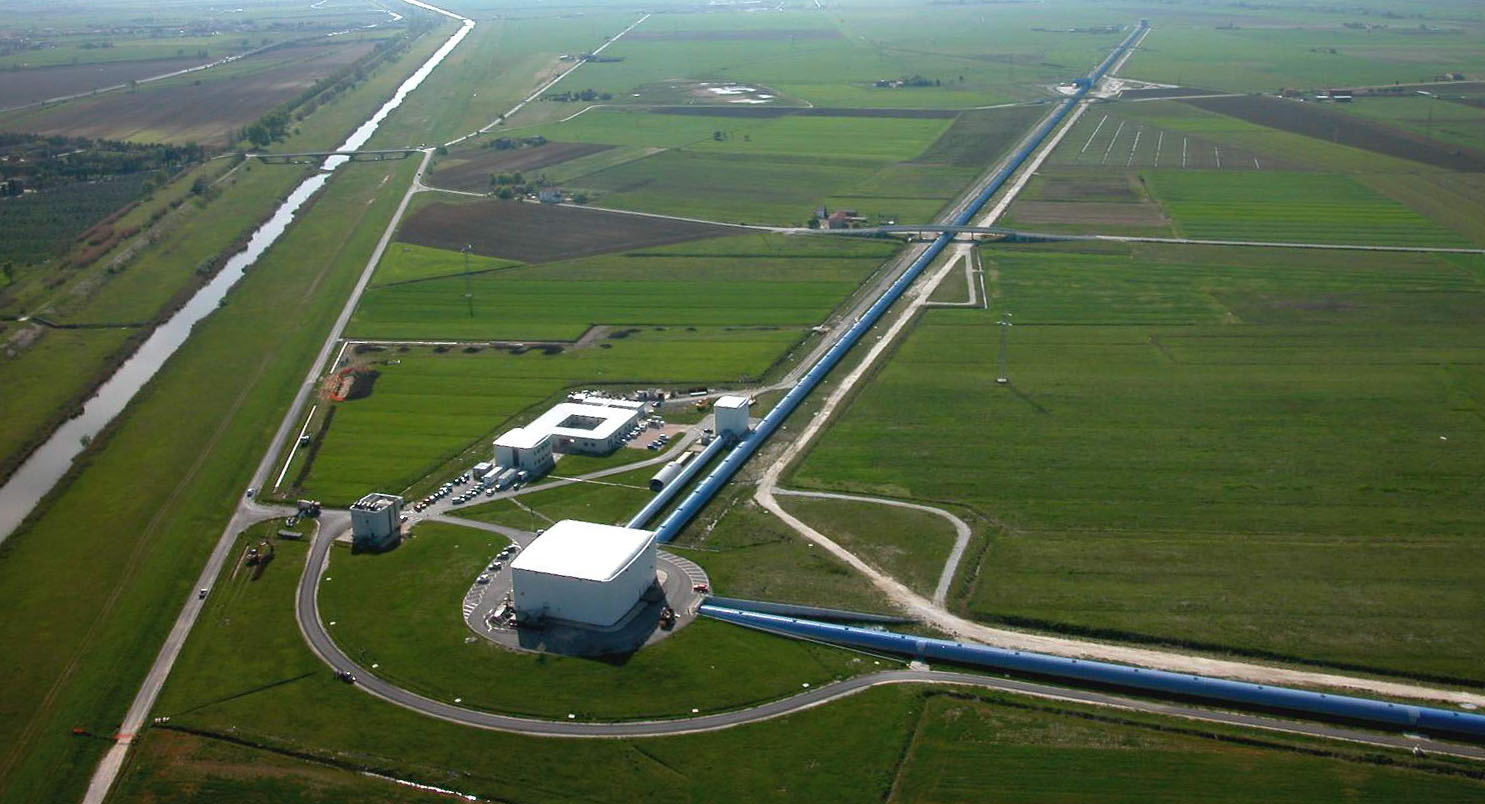
\includegraphics[width=\linewidth]{virgo}
			\captionof{figure}{Photo aérienne de l'interféromètre Virgo}
			\label{fig:virgo}
		\end{center}
	\end{minipage}
	\hfill
	\begin{minipage}[c]{.45\linewidth}
		~
		\begin{center}
			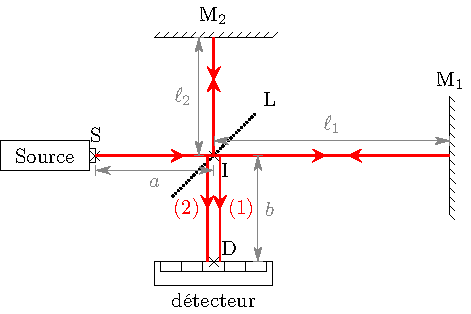
\includegraphics[width=\linewidth]{virgo_inter}
			\captionof{figure}{Schématisation de l'interféromètre}
			\label{fig:virgo_inter}
		\end{center}
	\end{minipage}

	Une source laser de longueur d'onde $\lambda = \SI{633}{\nano\meter}$ se
	trouve au point S et émet un faisceau de lumière le long de l'axe $(Ox)$. Ce
	faisceau laser est séparé en deux par une lame séparatrice L, qui divise
	l'amplitude d'un signal la rencontrant par 2. On considère alors que la moitié
	de la lumière entre dans le bras 1 et l'autre moitié dans le bras 2. Chaque
	faisceau ainsi obtenu parcourt un bras de l'interféromètre, est réfléchi sur
	un miroir (M$_1$ ou M$_2$) et revient vers la séparatrice.
	\bigbreak
	Le faisceau est recombiné par la séparatrice et le signal résultant est
	détecté par le détecteur D. La source laser émet au point S un signal de la
	forme $A \cos (\wt)$. Les deux bras de l'interféromètre ont pour longueur
	respectives $\ell_1$ et $\ell_2$. La distance entre la source S et la
	séparatrice est noté $a$ et la distance entre la séparatrice et le détecteur
	D est notée $b$.
	\bigbreak
	On négligera toute diminution de l'amplitude de l'onde lumineuse au cours de
	sa propagation (sur la Figure~\ref{fig:virgo_inter}, les rayons incidents et
	réfléchis sont décalés dans les bras de l'interféromètre pour améliorer la
	lisibilité de la figure~; en pratique, les rayons sont superposés).
}

\QR[6]{%
	Quelles sont les conditions pour que 2 ondes interfèrent~?
	Expliquer en détail la nécessité de faire des interférences lumineuses avec
	une unique source.
}{%
	Pour interférer, il faut que deux ondes soient \textbf{de même nature} \pt{1}
	et \textbf{de même fréquence} \pt{1}.
	\smallbreak
	Les sources lumineuses ont une phase à l'origine qui varie \pt{1}
	aléatoirement sur un temps très court, appelé \textbf{temps de cohérence}
	\pt{1}, bien plus petit que le temps d'acquisition des capteurs classiques~:
	on dit qu'elles émettent des \textbf{trains d'onde} \pt{1}.
	\smallbreak
	Pour pouvoir interférer de manière continue dans l'espace, il faut que les
	ondes aient la \textbf{même phase à l'origine} ($\Delta{\f_0} = 0$ \pt{1}),
	sinon l'intensité moyenne du signal serait nulle. On utilise pour cela une
	unique source.
}

\QR[2]{%
	Exprimer la distance parcourue par le rayon qui effectue le parcours (SD)$_1$
	se réfléchissant sur M$_1$ en fonction de $a$, $\ell_1$ et $b$.
}{
	\[
		\boxed{
			({\rm SD})_1 \stm[-1]{=}
			({\rm SI}) + ({\rm IM_1}) + ({\rm M_1I}) + ({\rm ID}) \stm[-1]{=}
			a+2\ell_1 + b
		}
	\]
}

\QR[5]{%
	En déduire l'expression du signal $s_1$ au point $D$ de l'onde lumineuse ayant
	effectuée le parcours (SD)$_1$. Comment s'appelle la valeur $\w/c$~?
}{
	Le signal met une durée $\Delta t_1 \stm[-1]{=}(a+2\ell_1 + b)/c$ pour aller
	de la source au détecteur. De plus, la moitié du signal est pe\stk(un){r}du à
	chaque fois que le faisceau traverse la lame semi-réfléchissante. Finalement
	\[
		s_1(t) \stm{=}
		\frac{A}{4}\cos(\omega (t- \Delta t_1) ) =
		\frac{A}{4}\cos(\omega (t- \frac{a+2\ell_1 + b}{c}) ) \stm{=}
		\boxed{\frac{A}{4}\cos(\wt- k(a+2\ell_1 + b))}
	\]
	avec $k \stm{=} \frac{\w}{c}$ le vecteur d'onde.
}

\QR[1]{%
	Exprimer la distance parcourue par le rayon qui effectue le parcours (SD)$_2$
	se réfléchissant sur M$_2$ en fonction de $a$, $\ell_2$ et $b$.
}{
	\[
		\boxed{
			({\rm SD})_2 =
			({\rm SI}) + ({\rm IM_2}) + ({\rm M_2I}) + ({\rm ID}) \stm{=}
			a+2\ell_2 + b
		}
	\]
}

\QR[1]{%
	En déduire l'expression du signal $s_2$ au point $D$ de l'onde lumineuse ayant
	effectue le parcours (SD)$_2$.
}{
	De la même manière,
	\[
		\boxed{s_1(t) \stm{=} \frac{A}{4}\cos(\wt- k(a+2\ell_2 + b))}
	\]
}

\enonce{
	\noindent On rappelle la formule d'addition~:
	\[
		\cos p + \cos q =
		2\cos \left( \frac{p+q}{2} \right)
		\cos \left( \frac{p-q}{2} \right)
	\]
}

\QR[3]{%
	Déterminer l'expression du signal lumineux total $s(t)$ mesuré par le
	détecteur au point D.
}{
	\begin{align*}
		s(t) & \stm[-1]{=} \frac{A}{4}\left(
		\cos\left(\wt- k(a+2\ell_1+b) \right)
		+
		\cos\left(\wt- k(a+2\ell_2+b) \right)
		\right)
		\\\Lra
		s(t) & \stm[-1]{=} \frac{A}{2}\left(
		\cos\left(
			\wt - \frac{k}{2}(a+2\ell_1+b) - \frac{k}{2}(a+2\ell_2+b)
			\right)
		\times
		\cos\left(
			- \frac{k}{2}(a+2\ell_1+b) + \frac{k}{2}(a+2\ell_2+b)
			\right)
		\right)
		\\\Lra
		\Aboxed{
		s(t) & \stm[-1]{=} \frac{A}{2}\left(
			\cos\left( \wt- k(a+\ell_1+\ell_2+b) \right)
			\times
			\cos\left(k (\ell_2-\ell_1)  \right)
			\right)
		}
	\end{align*}
}

\QR[3]{%
	Proposer une condition sur $\ell_1$ et $\ell_2$ pour que les deux signaux
	$s_1$ et $s_2$ soient en quadrature de phase au niveau du détecteur.
}{
	On veut $k(\ell_2-\ell_1) \stm[-1]{=} \pi/2$. Avec $k \stm[-1]{=}
		2\pi/\lambda$~:
	\[
		\frac{2\pi(\ell_2-\ell_1)}{\lambda} = \frac{\pi}{2}
		\qquad \Rightarrow \qquad
		\boxed{\ell_2-\ell_1 \stm[-1]{=} \frac{\lambda}{4}}
	\]
}

\enonce{
	Lors du passage d'une onde gravitationnelle, les bras de l'interféromètre se
	déforment. Les longueurs $\ell_1$ et $\ell_2$ varient alors en fonction du
	temps.
}

\QR[2]{%
	Expliquer comment cet interféromètre permet de détecter le passage d'une onde
	gravitationnelle.
	\smallbreak
	Qu'observe-t-on au niveau du détecteur ?
}{
	Quand il y a une onde gravitationnelle, les longueurs $\ell_2$ et $\ell_1$ ne
	varient pas de la même façon et $(\ell_2-\ell_1)$ varie. On voit donc une
	variation du signal en $D$ qui est maximum quand les 2 ondes sont en phase
	(interférence constructives) et minimale quand les 2 ondes sont en opposition
	de phase (interférences destructives).
}

\end{document}
